% Autor: Leonhard Segger, Alexander Neuwirth
% Datum: 2017-10-30
\documentclass[
	% Papierformat
	a4paper,
	% Schriftgröße (beliebige Größen mit „fontsize=Xpt“)
	12pt,
	% Schreibt die Papiergröße korrekt ins Ausgabedokument
	pagesize,
	% Sprache für z.B. Babel
	ngerman
]{scrartcl}

% Achtung: Die Reihenfolge der Pakete kann (leider) wichtig sein!
% Insbesondere sollten (so wie hier) babel, fontenc und inputenc (in dieser
% Reihenfolge) als Erstes und hyperref und cleveref (Reihenfolge auch hier
% beachten) als Letztes geladen werden!

% Silbentrennung etc.; Sprache wird durch Option bei \documentclass festgelegt
\usepackage{babel}
% Verwendung der Zeichentabelle T1 (Sonderzeichen etc.)
\usepackage[T1]{fontenc}
% Legt die Zeichenkodierung der Eingabedatei fest, z.B. UTF-8
\usepackage[utf8]{inputenc}
% Schriftart
\usepackage{lmodern}
% Zusätzliche Sonderzeichen
\usepackage{textcomp}

% Mathepaket (intlimits: Grenzen über/unter Integralzeichen)
\usepackage[intlimits]{amsmath}
% Ermöglicht die Nutzung von \SI{Zahl}{Einheit} u.a.
\usepackage{siunitx}
% Zum flexiblen Einbinden von Grafiken (\includegraphics)
\usepackage{graphicx}
% Abbildungen im Fließtext
\usepackage{wrapfig}
% Abbildungen nebeneinander (subfigure, subtable)
\usepackage{subcaption}
% Funktionen für Anführungszeichen
\usepackage{csquotes}
% Zitieren, Bibliographie
\usepackage{biblatex}


% Zur Darstellung von Webadressen
\usepackage{url}
%chemische Formeln
\usepackage[version=4]{mhchem}
% siunitx: Deutsche Ausgabe, Messfehler getrennt mit ± ausgeben
\usepackage{floatrow}
\floatsetup[table]{capposition=top}
\usepackage{float}
% Verlinkt Textstellen im PDF-Dokument
\usepackage[unicode]{hyperref}
% "Schlaue" Referenzen (nach hyperref laden!)
\usepackage{cleveref}
\sisetup{
	locale=DE,
	separate-uncertainty
}
\bibliography{6Mi_E2_10-01-2018_References}

\begin{document}
	
	\begin{titlepage}
		\centering
		{\scshape\LARGE Versuchsbericht zu \par}
		\vspace{1cm}
		{\scshape\huge E2 - Millikan \par}
		\vspace{2.5cm}
		{\LARGE Gruppe 6Mi \par}
		\vspace{0.5cm}
		
		{\large Alexander Neuwirth (E-Mail: a\_neuw01@wwu.de) \par}
		{\large Leonhard Segger (E-Mail: l\_segg03@uni-muenster.de) \par}
		\vfill
		
		durchgeführt am 10.01.2018\par
		betreut von\par
		{\large Johann Preuß}
		
		\vfill
		
		{\large \today\par}
	\end{titlepage}
	\tableofcontents
	\newpage
	
	\section{Kurzfassung}
	%TODO Hypothese	und deren Ergebnis
	%TODO Ergebnisse, auch Zahlen, mindestens wenn's halbwegs Sinn ergibt
	%TODO Was wurde gemacht
	%TODO Rechtschreib mal gucken, weil nur so gefreestyled (@myself)
	Durch den Millikan Versuch soll die Elemtentarladung bestimmt werden.
	Dies gelingt dadurch, dass man die Bewegung von Öltröpfchen in einem konstantem elektrischen Feld beobachtet.
	Einfluss auf die Bewegung nimmt die Gravitation, Luftreibung, Coulomb-Kraft und der Auftrieb.
	Da ein direktes Vermessen des Öltröpfchens nicht praktikabel ist, werden zwei Fälle untersucht.

	Beim ersten wird die Zeit für eine bestimmte Strecke gemessen, wobei das elektrische Feld parallel zum Gravitationsfeld ausgerichtet ist. 
	Im zweiten Fall ist das elektrische Feld ausgeschaltet, sodass sich aus beiden Messugen Ladung und Radius des Tröpfchens bestimmen lassen.
	Die Ladung der Öltröpfchen entsteht durch Reibung beim Einsprühen in den Kondensator. 
	Wenn es eine Elementarladung gibt, müssten die Tröpfchen stets mit einem Vielfachen derer geladen sein. %TODO Hypothese e- Theorie wert
	%TODO ERgebnisse
	%TODO mehr? 


	\section{Voüberlegungen}
	Zur Vorbereitung auf den Versuch wurden folgende Aufgaben bearbeitet:
	\begin{itemize}
		\item Skizze der Kräftegleichgewichte wurde vor dem Experiment angezeichnet und besprochen.
		\item Herleitung der Kräftegleichgewichte aus den Formeln für $ r $ und $ Q $: %TODO
		\item Schätzung der Dauer der Beschleunigungsphase eines Tröpfchens %TODO
		\item Es ist wichtig die Kondensatorplatten waagerecht auszurichten, weil sie einerseits parallel zu einander sein müssen, damit das elektrische Feld möglichst homogen ist und andererseits muss die Kraft des elektrischen Feldes parallel zur Gravitationskraft und damit allen anderen Kräften sein.
		\item Es werden Öltröpfchen anstelle von Wassertröpfchen verwendet, weil Öl deutlich weniger flüchtig ist, man also keinen Massenverlust der Tröpfchen während der Beobachtung mit einbeziehen muss.
		\item Im elektrischen Feld steigen stärker geladene Teilchen schneller auf als weniger geladene. Deshalb muss man, um stärker und weniger stark geladene Teilchen bei gleicher Geschwindigkeit zu beobachten, bei stärker geladenen Teilchen die Spannung verringern und umgekehrt sie bei schwächer geladenen erhöhen.
		\item Man sollte die einzelnen Messungen nicht innerhalb der Stoppuhr aufsummieren, weil dies bedeuten würde, dass wenn man sich bei einer der Messungen vermisst, alle bisherigen Messungen dieses Teilchens wiederholen müsste, während man ansonsten nur die eine misslungene erneut durchführen muss.
		\item Bei steigender Temperatur steigen mittlere Weglänge $ \lambda $ und Viskosität $ \eta $ in Luft (siehe Literaturwerte aus der Anleitung). %TODO Amazon-Reflink in der Videobeschreibung
		Dies ist nicht in allen Medien der Fall.
	\end{itemize}
	
	\section{Methoden}
	%TODO Bilder von der Website klauen
	In \cref{Millikan} ist er Aufbau des Experiments illustriert.
	Um die Öltröpfchen erkennbar zu machen wurde der Raum abgedunkelt und die Beleuchtungseinrichtung eingeschaltet.
	Zunächst wurden an den Kondensatorplatten eine Gleichspannung von ca. \SI{600}{V} angelegt. 
	Darauf wurden Öltröpfchen in das elektrische Feld gesprüht.
	Mit einem Mikroskop war nun erkennbar, dass ein Töpfchen welches ansteigt, geladen ist. 
	Durch die Linsen des Mikroskops ist Bild seitenverkehrt, folglich hatte es den Anschein, dass sich das Öltropfchen nach unten bewegt. 
	Nachdem man eine Tröpfchen gefunden hatte, wurde das Feld ausgeschaltet und die Zeit gemessen die das Tröpfchen für eine Fall von zwei Skalenteilen (\SI{0,2}{mm}) benötigte. 
	Dann wurde das elektrische Feld wieder eingeschaltet und die selbe Messung wurde erneut durch geführt mit umgekehrter Bewegung des Teilchens.
	Diese zwei Messungen wurden mehrfach für jedes Tröpfchen durchgeführt. 
	Zu Beachten galt es, dass Luftstömungen die Tröpfchen beeinflussen können, desshalb wurde der Raum zwischen den Kondensatorplatten mit einem Stück Pappier zwischen Ölzerstäuber und Einsprühöffnung abgeschlossen.
	Außerdem steigt der Fehler mit der Ladung $Q$, wesshalb man bereits während des Experiments die Ladung einzelner Tröpfchen berechnet, um diese möglichst klein halten zu können.
	%TODO mehr!


	\begin{figure}[H]
		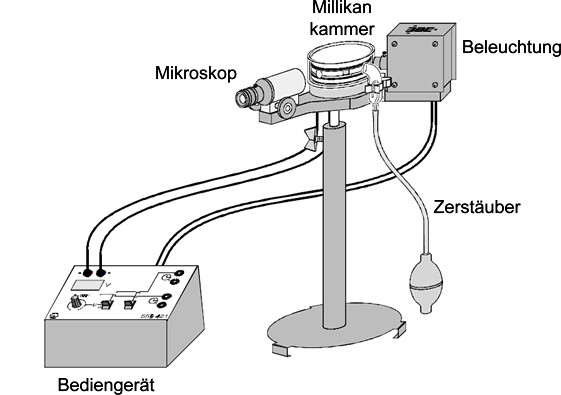
\includegraphics[width=0.7\textwidth]{Millikan}
		\centering
		\caption{Exemplarischer Aufbau des Millikan Versuchs. \protect\footnotemark}
		\label{Millikan}
		\centering
	\end{figure} 
	\footnotetext{Grafik von \citetitle{TUM}\cite{TUM}}

	
	\section{Ergebnisse und Diskussion}
	%TODO Datenanalyse -> Überschrift?
	%TODO Unsicherheiten
	

	\subsection{Beobachtung}
	\subsubsection*{Technische Daten und Konstanten} %TODO Amazon-Reflink in der Videobeschreibung
	\begin{itemize}
		\item Plattenabstand: $d=\SI{6 \pm 0,05}{mm}$
		\item Okularvergrößerung: 10
		\item Objektivvergrößerung: \SI{2 \pm 0,05}{}
		\item Länge der Mikrometerskala: \SI{10}{mm}
		\item kleine Skalenteilung: \SI{0,1}{mm}
		\item Öldichte: $\rho_\text{Öl} = \SI{874 \pm 1,2}{\kilogram \per \metre \cubed} $ (gemäß der Temperaturabhängigkeit der Dichte bei unbekannter exakter Temperatur nahe Raumtemperatur von \SI{20}{\degreeCelsius}mit rechteckiger WDF)
		\item Dynamische Viskosität der Luft: $\eta = \SI{18,2 \pm 0,18}{\micro \pascal \second} $ (gemäß der Temperaturabhängigkeit der Dynamischen Viskosität bei unbekannter exakter Temperatur nahe Raumtemperatur von \SI{20}{\degreeCelsius} mit rechteckiger WDF)
		\item Dichte der Luft: $\rho_\text{L}= \SI{1,2929}{\kilogram \per \metre \cubed}$ (ohne Unsicherheit, denn gering gegenüber der Dichte von Öl und deren Unsicherheit)
		\item Ortsfaktor: \SI{9,81 \pm 0,02}{\meter \per \second \squared} (ortsabhänige Schwankung nach oben abgeschätzt)
	\end{itemize}
	Die Spannung zwischen den Kondensatorplatten wurde auf \SI{565}{V} eingestellt, sank aber während des Versuchs auf \SI{560}{V}.
	Die Unsicherheit der Digitalanzeige verschwindet gegen diese Schwankungen, deswegen wird (gemäß rechteckiger WDF) eine Spannung von \SI{562,5 \pm 0,8}{V} angenommen.
	Es wurde immer die Zeit gemessen, die die Tröpfchen für eine Strecke von zwei großen Skaleneinteilungen benötigt haben.
	Dabei entsprachen zwei große (20 kleine) Skaleneinteilungen  einer Strecke von \SI{2\pm 0,02}{mm} (\SI{0,2}{mm} Ableseungenauigkeit mit dreieckiger WDF).
	%Wenn man diese Länge gemäß der Okular- und Objektivvergrößerung gemäß \cref{Partielle_Unsicherheiten} umrechnet erhält man für die zurückgelegte Strecke der Tröpfchen \SI{100\pm 2,7}{\micro \meter}.
	Für die Zeitmessung mithilfe der Stoppuhr ergibt sich die Unsicherheit aus der kombinierten Unsicherheit der Digitalanzeige der Stoppuhr und der Reaktionszeit des Menschen gemäß der Gleichung zur Kombination von Unsicherheiten. %TODO ref wen nötig
	Dabei schätzen wir die Reaktionszeit des Menschen aufgrund der teilweise schwierigen Erkennbarkeit der Tropfen nach oben mit \SI{0.2}{s} ab.
	Dieser Fehler überlagert deutlich die Unsicherheit von \SI{0.006}{s} durch die Digitalanzeige (zwei Nachkommastellen mit rechteckiger WDF).
	Dann wurde aus den Zeitmessungen der Mittelwert der Fall- und Steigzeit für jedes der 15 Tröpfchen gebildet.
	Die Unsicherheit dieser Mittelwerte ergibt sich aus der kombinierten Unsicherheit aus Standardunsicherheit und einem Fünftel des zuvor genannten Fehlers der Stoppuhr.
	
	\begin{equation}
	u(y) = \sqrt{  \sum_{i=0}^{N} \left( \frac{\partial f}{\partial x_i}u(x_i)\right)^2  }
	\label{Partielle_Unsicherheiten}
	\end{equation}
	Die Ladungen der Öltröpfchen wurden mithilfe von \cref{Ladung} bestimmt und die kombinierte Unsicherheit der Ladung mit \cref{Ladung} und \cref{Partielle_Unsicherheiten} und in \cref dargestellt. %TODO reflink Grafik
	\begin{equation}
		Q=\frac{18 \pi d}{U} \sqrt{\frac{\eta^3 v_\downarrow}{2(\rho_\text{Öl}-\rho_\text{L})g}}(v_\downarrow + v_\uparrow)
		\label{Ladung}
	\end{equation}
	%TODO Stokesscher Satz korrektur

	\subsection{Diskussion}
	%TODO Bezug/Nutzten oder sonst was
	%TODO auch hier die Hypothese wiederholen
	%TODO bezug auf unsicherheiten
	Der Literaturwert für die Elementarladung beträgt \SI{1,6021766208 \pm 0,0000000098 e-19}{C} \cite{Elementarladung}.
	
	\section{Schlussfolgerung}
	Zusätzlich hätte man die Ladung auch durch ein genaues Einstellen der Spannung bestimmen können, dies ist aber unpraktisch, da die Spannung am Kondensator nicht ausreichend genau angegeben ist.
	Außerdem wäre nach wie vor der Radius des Tröpfchen durch eine andere Methode zu bestimmen.
	%TODO Rückgriff auf Hypothese und drittes Nennen dieser
	%TODO Millikan e/2 möglich  aber unwahrscheinlich
	%TODO nichts zu falsifizeiren
	
	%TODO Quellen zitieren, Websiten mit Zugriffsdatum
	%TODO Verweise auf das Laborbuch (sind erlaubt)
	%TODO Tabelle + Bilder mit Beschriftung

	\printbibliography
\end{document}
